% -*- Mode: LaTeX -*-
\documentclass[pdflatex,colorlinks,landscape]{beamer}
% $Id: ErrorCorrection.tex,v 1.178 2023/01/24 14:27:53 marek Exp $
\mode<presentation>{
  % \usetheme{plain}
  %\usetheme{Warsaw}
  \usetheme{Hannover}
  % \usetheme{Dresden}
  % or ...

  \setbeamercovered{transparent}
  % or whatever (possibly just delete it)
}

\date{February 18, 2023}
\usepackage{etex}
\usepackage{mathtools}
\usepackage{MnSymbol}

\usepackage[english]{babel}
% or whatever

\usepackage[latin1]{inputenc}
% or whatever

\usepackage{times}
\usepackage[T1]{fontenc}
% Or whatever. Note that the encoding and the font should match. If T1
% does not look nice, try deleting the line with the fontenc.

%% Include graphics
\usepackage{graphicx}

%% To wrap text around images
\usepackage{wrapfig}

%% For typesetting algorithms
% \usepackage{algorithmic}
\usepackage{algorithmicx}

%% For inclusion of PostScript
\usepackage{epsfig}

%% For inclusion of PicTeX pictures
% \usepackage{pictex}

%% For drawing trees
\usepackage{tikz}
\usepackage{tikz-qtree}

\usepackage{listings} %typesets code
\usepackage{color} %red, green, blue, yellow, cyan, magenta, black, white
\definecolor{mygreen}{RGB}{28,172,0} % color values Red, Green, Blue
\definecolor{mylilas}{RGB}{170,55,241}

\lstset{language=Matlab,%
  % basicstyle=\color{red},
  breaklines=true,%
  morekeywords={matlab2tikz},
  keywordstyle=\color{blue},%
  morekeywords=[2]{1}, keywordstyle=[2]{\color{black}},
  identifierstyle=\color{black},%
  stringstyle=\color{mylilas},
  commentstyle=\color{mygreen},%
  showstringspaces=false,%without this there will be a symbol in the places where there is a space
  numbers=left,%
  numberstyle={\tiny \color{brown}},% size of the numbers
  numbersep=9pt, % this defines how far the numbers are from the text
  emph=[1]{if,elseif,else,for,end,break,parfor},emphstyle=[1]\color{red}, %some words to emphasise
  % emph=[2]{word1,word2}, emphstyle=[2]{style},    
}



% For algorithms
\usepackage{algorithmicx}
\usepackage{algorithm}
\usepackage{algpseudocode}

\algnewcommand\RETURN{\algorithmicreturn}
\algnewcommand\PROCEDURE{\item[\algorithmicprocedure]}%
\algnewcommand\algorithmicendprocedure{\textbf{end procedure}}
\algnewcommand\ENDPROCEDURE{\item[\algorithmicendprocedure]}%
\algnewcommand{\algvar}[1]{{\text{\ttfamily\detokenize{#1}}}}
\algnewcommand{\algarg}[1]{{\text{\ttfamily\itshape\detokenize{#1}}}}
\algnewcommand{\algproc}[1]{{\text{\ttfamily\detokenize{#1}}}}
\algnewcommand{\algassign}{\leftarrow}
\algnewcommand\algorithmicfalse{\textbf{false}}
\algnewcommand\FALSE{\algorithmicfalse}
\algnewcommand\algorithmictrue{\textbf{true}}
\algnewcommand\TRUE{\algorithmictrue}

\usepackage{fancyvrb}

% For captions anywhere
\usepackage{caption,subcaption}

% For exact sequences
\usepackage[all,cmtip]{xy}

% ----------------------------------------------------------------%
% FILE-LOCAL DEFINITIONS
% ----------------------------------------------------------------%


\def\ints{\mathbb Z}		% ints in math mode only
\def\nats{\mathbb N}		% ints in math mode only
\def\rats{\mathbb Q}		% rational numbers in math mode only
\def\reals{\mathbb R}		% reals in math mode only
\def\complex{\mathbb C}		% complex in math mode only
\def\disk{\mathbb D}		% unit disk in math mode only
\def\torus{\mathbb T}		% torus in math mode only
\def\proj{\mathbb P}		% projective space in math mode only

\def\reducesto#1{{\mathop{\longrightarrow}\limits_{#1}}}
\def\implies{\Rightarrow}
\def\Id{\mathrm{Id}}
\def\Prob{\mathrm{Prob}}
\def\Expect{\mathbb{E}}
\def\calC{\mathcal{C}}
\def\calD{\mathcal{D}}
\def\F{\mathbb{F}}
\def\P{\mathbb{P}}

\renewcommand\vec[1]{\mathbf{#1}} % Vector
\newcommand\mat[1]{\mathbf{#1}} % Matrix

\renewcommand\emph[1]{{\color{magenta}#1}}

% ----------------------------------------------------------------%
%								 % 
% TITLE PAGE						 %
%								 % 
% ----------------------------------------------------------------%

% ----------------------------------------------------------------
\title[Parallelism]{Parallel Programing}
\subtitle{With MATLAB Examples}

% ----------------------------------------------------------------
\author{Marek Rychlik}

\institute[University of Arizona]{
  Department of Mathematics\\
  University of Arizona
}
% ----------------------------------------------------------------


\graphicspath{{images/}}

% ----------------------------------------------------------------%
%								 % 
%	BEGINNING OF SLIDES					 %
%								 % 
% ----------------------------------------------------------------%

% ----------------------------------------------------------------
\begin{document}
% ----------------------------------------------------------------

\begin{frame}
  \titlepage
\end{frame}

\section{OS Parallelism}

\begin{frame}{Parallelism in the OS}
  \begin{itemize}
  \item A modern OS has a multitude of processes running, as shown by a \emph{system
      monitor}
  \item OS creates {\color{red}an illusion of parallelism} even if it runs on a single CPU
    not capable of multi-threading in hardware.
  \end{itemize}
  \begin{figure}
    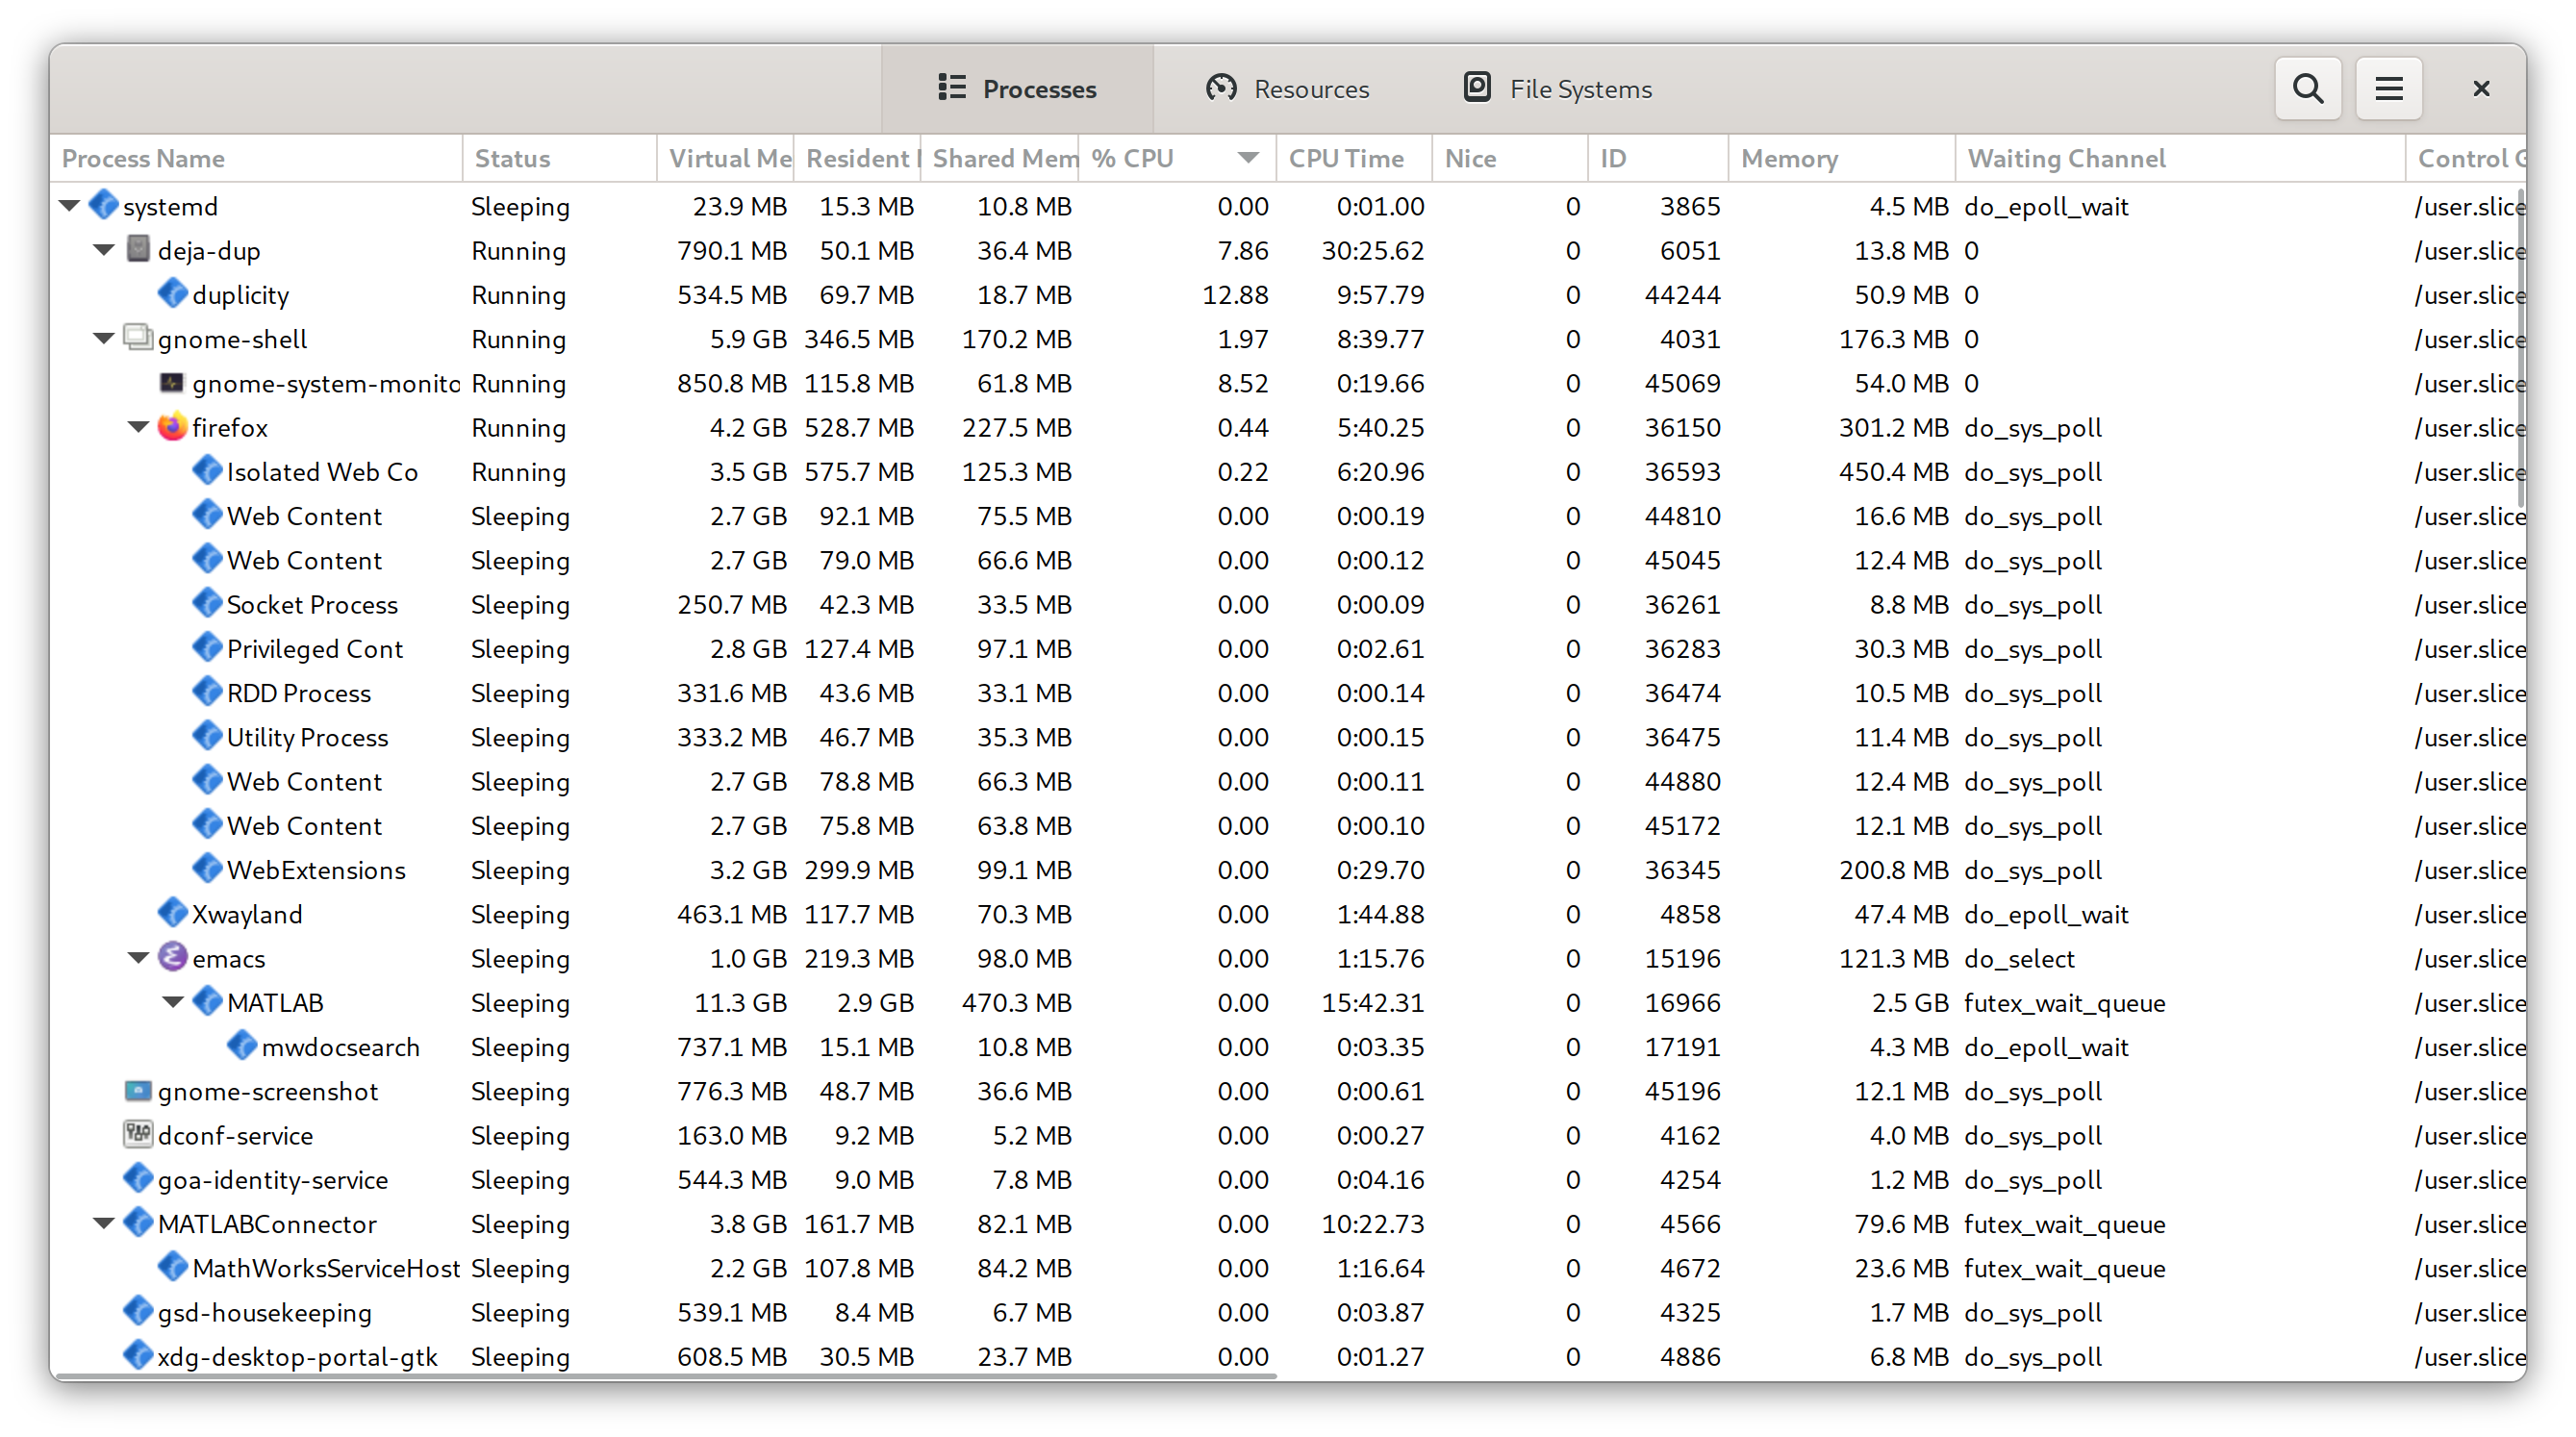
\includegraphics[width=.9\textwidth]{SystemMonitor.png}
    \caption{\href{https://askubuntu.com/questions/19442/what-is-the-waiting-channel-of-a-process}{Explanations}}
  \end{figure}
\end{frame}

\begin{frame}{How many CPUs/Hardware threads do I have?}
  \begin{figure}
    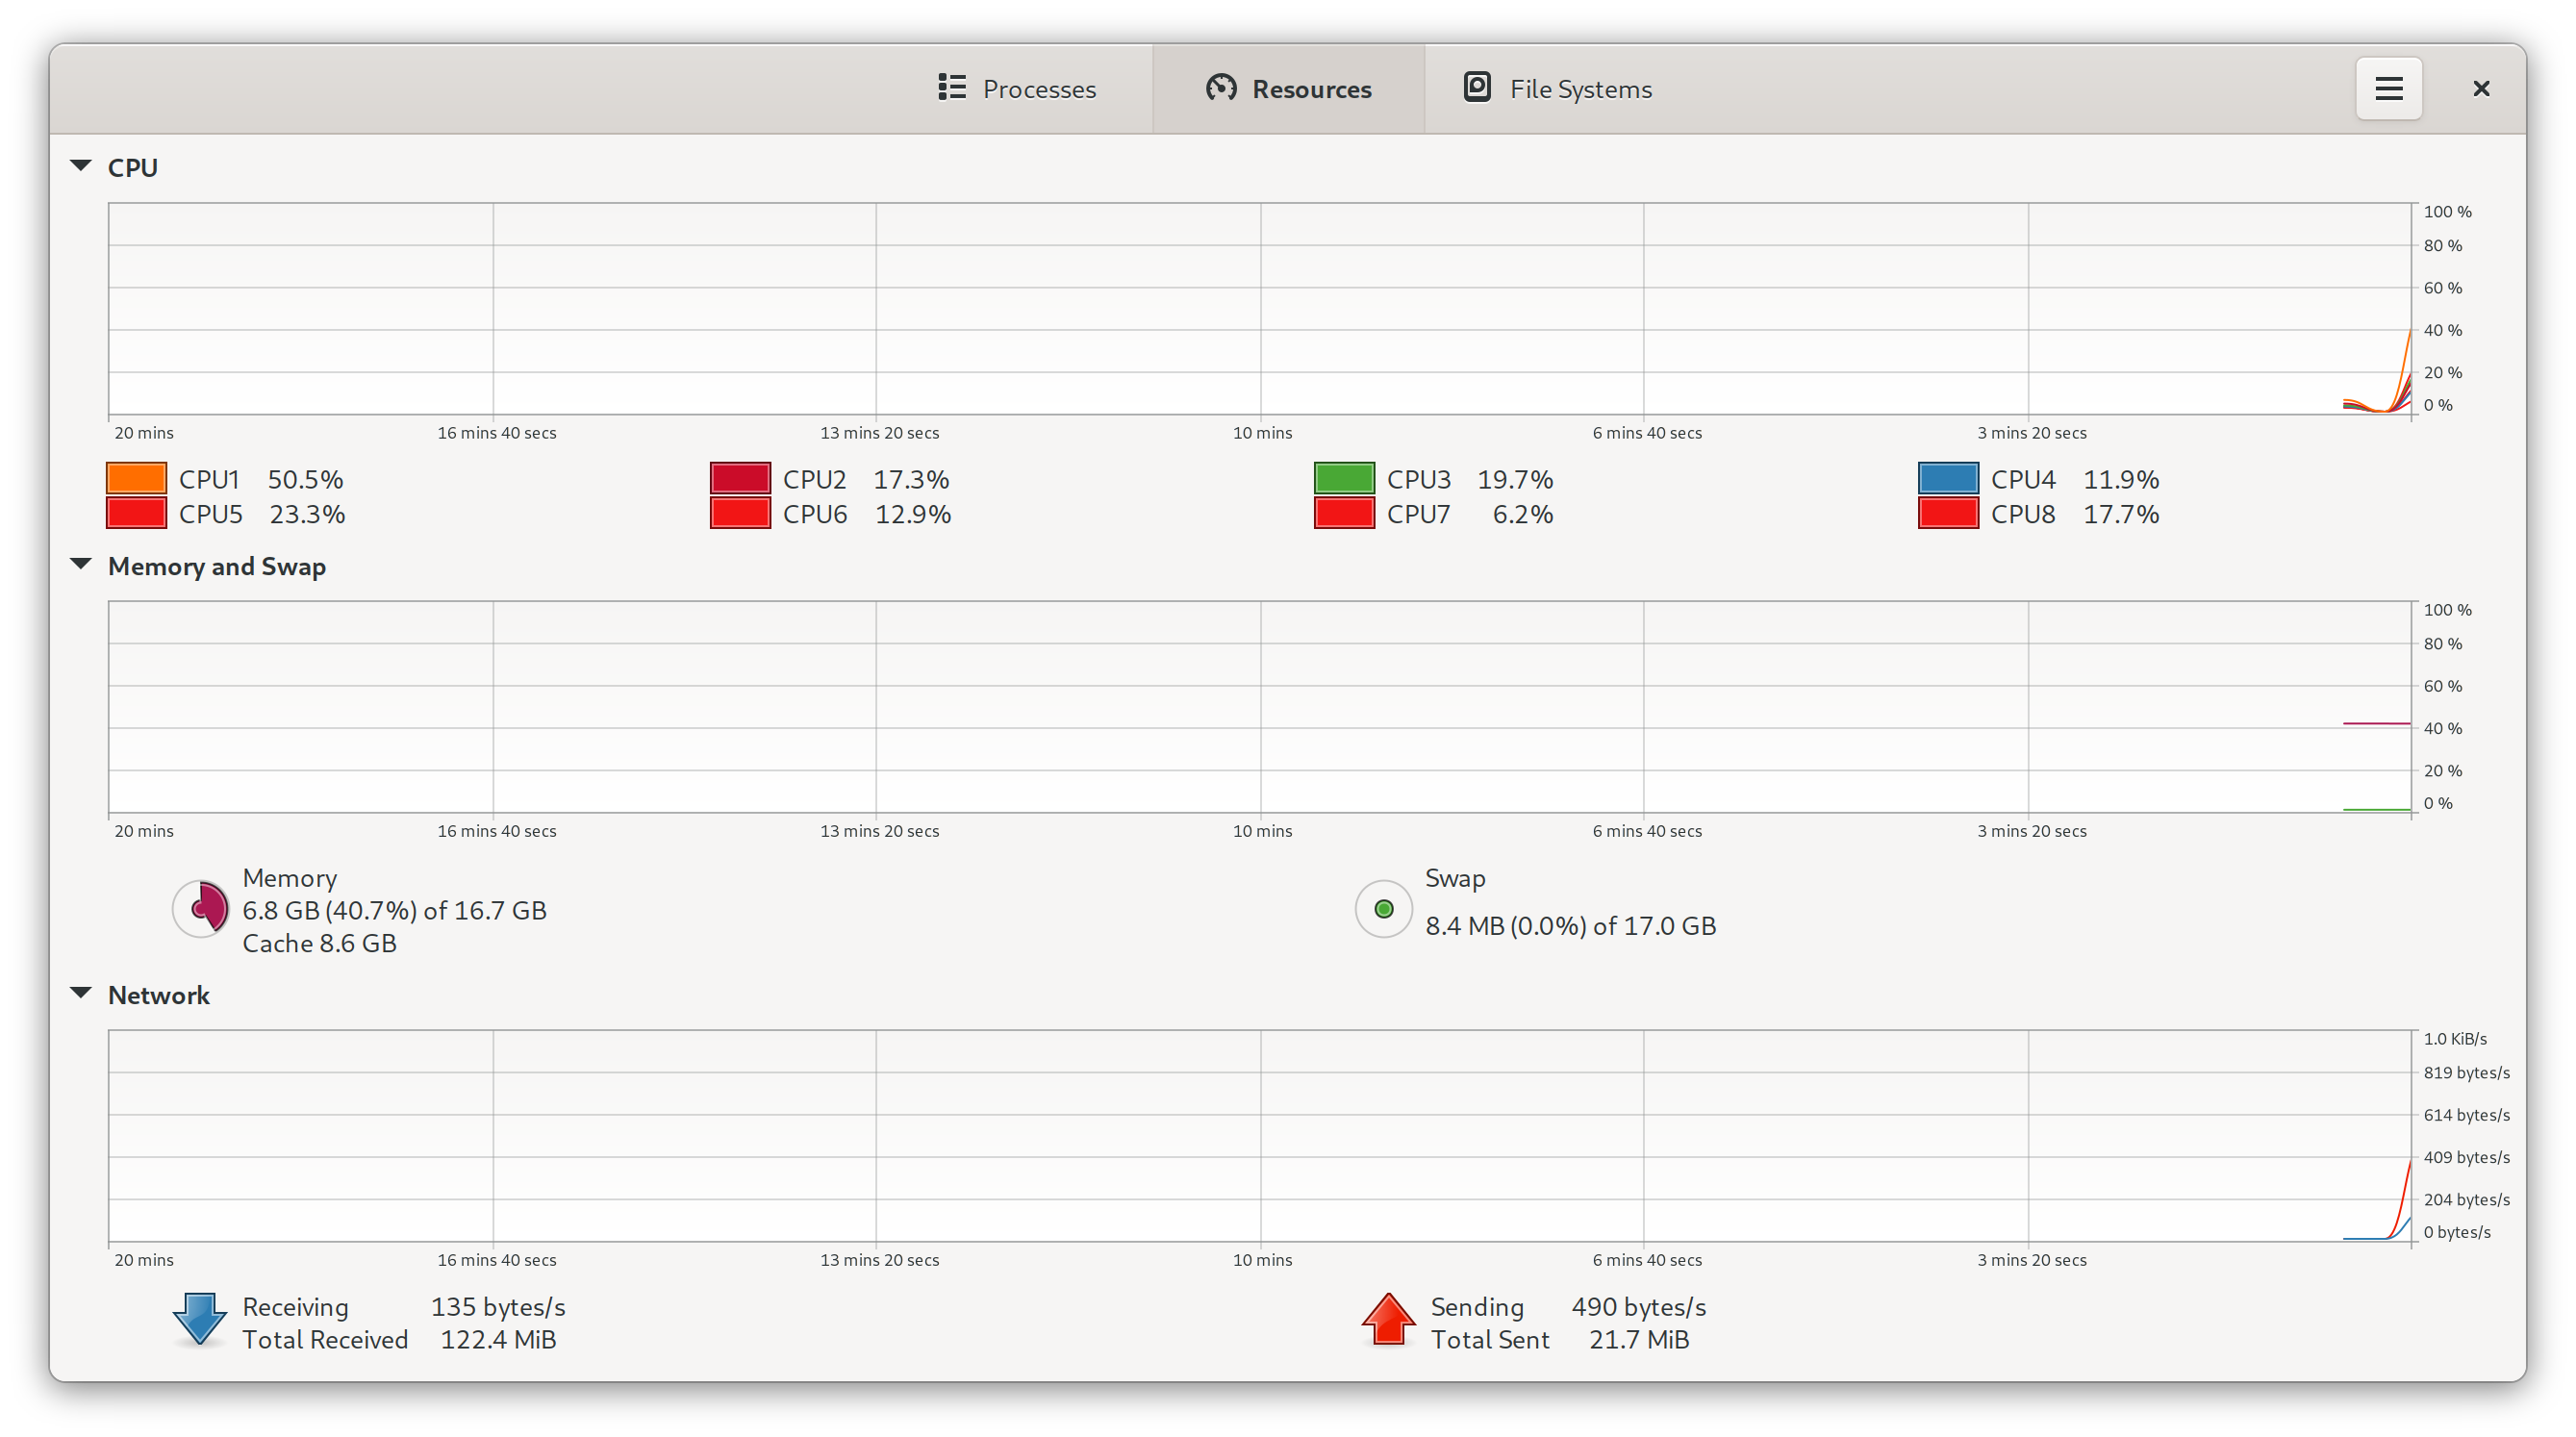
\includegraphics[width=\textwidth]{Resources.png}
  \end{figure}
\end{frame}

\begin{frame}{Forking in Bash (\&) --- a minimal variant}
  \lstinputlisting[language=Bash]{forkme_simple.sh}
\end{frame}
  
\begin{frame}[allowframebreaks]{Forking in Bash (\&)}
  \begin{small}
    \lstinputlisting[language=Bash]{forkme.sh}
  \end{small}
  \VerbatimInput{outputs/forkme_output.txt}
\end{frame}

\begin{frame}{A remarkable, more rare output}
  \VerbatimInput{outputs/forkme_output_rare.txt}
\end{frame}


\begin{frame}[allowframebreaks]{A Glossary of Terms}
  \begin{description}
  \item[program counter] The location (address) of the instruction currently
    being executed; a place in a program
  \item[process] A running program with all necessary resources
    (program counter, open file descriptors, memory state)
  \item[fork, forking, clone] The UNIX/Linux \emph{system call}
    which allows one process to create another one
  \item[IPC, inter-process communication] The protocol by which
    two distinct processes can exchange information
  \item[thread (of execution)] Formerly known as \emph{a light-weight process}
    directly shares the state of memory (variables) with other
    threads; threads have \emph{separate program counters};
    a modern process is a \emph{collection of threads}
  \item[process/thread synchronization] Mechanisms by which
    one process tells another not to mess with some sensitive
    parts of its state; IPC can be used for proces synchronization;
    threads are synchronized by \emph{mutexes}
  \item[mutex, futex] A mutually exclusive lock, which a simple integer
    (logical) variable which is set/unset (=acquired/released) by a
    thread. What is important is the \emph{interpretation} by another
    thread.  A thread agrees not to do certain things when mutex is
    acquired by another, until it is released. \emph{Semaphores} generalize
    mutexes to arbitrary integer values. \emph{Futex} is a \emph{fast mutex},
    introduced by the Linux OS.
  \item[atomicity] Some operations need to be atomic, such as changing
    the value of a mutex/semaphore. Atomicity means that a thread that
    reads the value of a mutex does not get an inconsistent value
    while another thread is {\color{red} in the process of changing it}.
    Normal variables cannot be used as mutexes because reading
    and writing to them {\color{red}is not atomic}. Atomicity is implemented
    using hardware (special instructions) and compiler (awarness that some
    variables must be changed atomically).
  \end{description}
\end{frame}

\section{Trivial Parallelism}

\begin{frame}[allowframebreaks]{MATLAB 'parfor' (parallel for)}
  \begin{small}
    \lstinputlisting{MATLAB/parforEx.m}
  \end{small}
  \begin{tiny}
    \VerbatimInput{outputs/parforEx_output.txt}
  \end{tiny}
  \begin{block}{Question}
    Why does 'All done' print only once? Only at the end?
  \end{block}
\end{frame}

\begin{frame}{Parallel pools, workers, clusters}
  \begin{itemize}
  \item TIP: first  install \href{https://www.mathworks.com/products/parallel-computing.html}{Parallel
      Computing Toolbox} and try its GUI to configure a cluster
  \item \emph{Workers} are a MATLAB abstraction of threads, and
    they should directly map to hardware (CPU, hardware threads)
  \item A \emph{paralel pool} is a collection of workers under the
    management of the \emph{main thread}
  \item A parallel pool can live on one or more CPUs, and can be distributed
    across many computers; these details are abstracted away
  \item A \emph{cluster} is defined by a configuration file (a
    \emph{profile}, eg., 'local.settings') and it specifies computers
    and the number of CPU used on each machine. The configuration file
    must be placed in one of several standard places (see 'help
    parcluster').
  \end{itemize}
\end{frame}

\begin{frame}[allowframebreaks]{Accumulating values, reduction variables}
  \begin{small}
    \lstinputlisting{MATLAB/reductionVar.m}
  \end{small}
  \begin{tiny}
    \VerbatimInput{outputs/reduction_var_output.txt}
  \end{tiny}
  \begin{block}{Fact}
    Deterministic: the answer is always the same.
  \end{block}

  \begin{figure}
    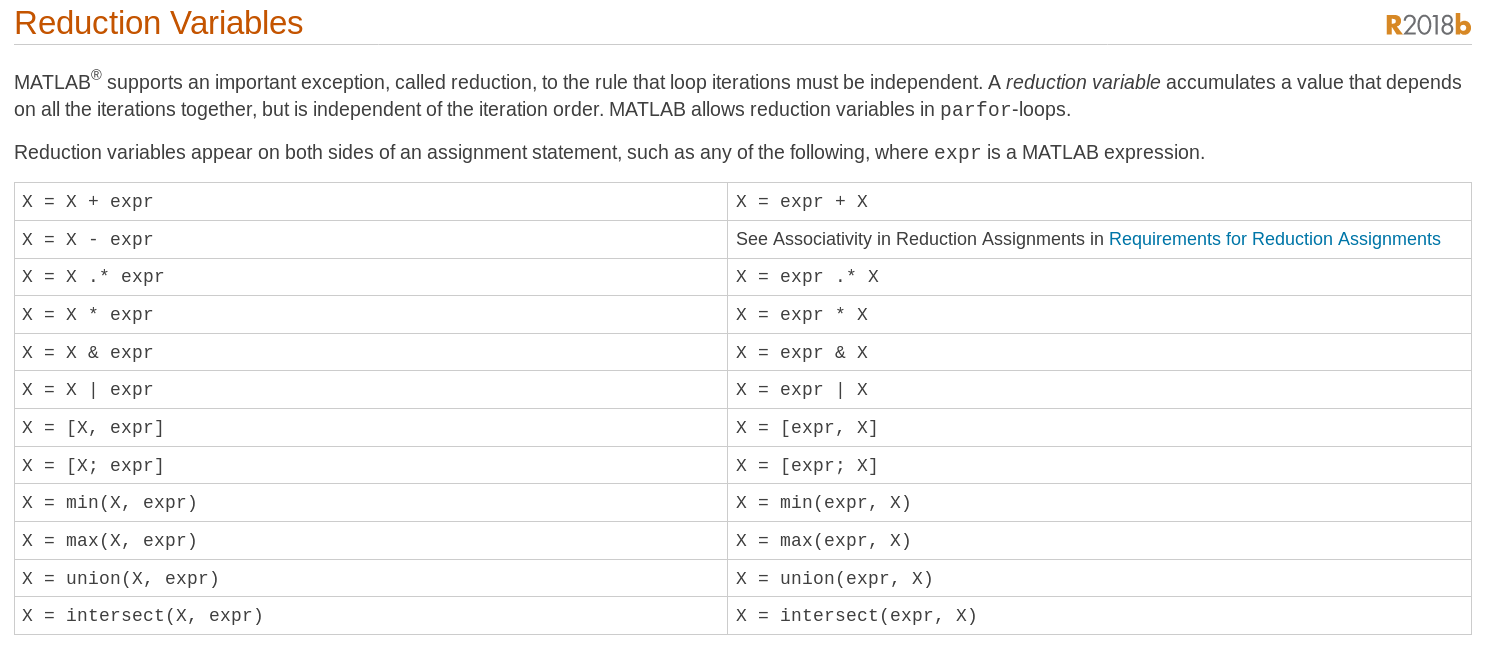
\includegraphics[width=\textwidth]{MATLAB/ReductionVariables.png}
  \end{figure}
\end{frame}

\section{An Intro to MPI}
\begin{frame}{SPMD and SIMD}
  \begin{description}
  \item[SPMD] Stands for ``Single program, multiple data''. \emph{Multiple
    autonomous processors} simultaneously execute the same program at
    independent points (program counters). Can be implemented on general
    purpose CPUs (Intel, AMD)
  \item[SIMD] Stands for ``Single-instruction, multiple data''.  A
    \emph{vector processor} processes the same instruction on different
    data (example: coordinatewise addition or multiplication of two
    vectors).
  \end{description}
  Modern CPU(s) implements \emph{both paradigms}:
  \begin{itemize}
  \item SIMD uses Intel/AMD \emph{SSE instructions} and \emph{vector registers};
  \item SPMD uses multiple \emph{threads}, \emph{cores} and CPUs.
  \end{itemize}
\end{frame}

\begin{frame}{The MPI (Message Passing Interface)}
  \begin{itemize}
  \item The most successful realization of SPMD; used in MATLAB; 40 years of history 
  \item Implementations in C, C++, Fortran exist, with high-level
    language interfaces
    (e.g., \href{https://mpi4py.readthedocs.io/en/stable/}{Python}).
  \item Worker becomes a \emph{lab}
  \item Worker knows its identity, or \emph{labindex}
  \item The main thread is now a lab with \emph{labindex==1} (recall: MATLAB has 1-based arrays)
  \item Labs communicate by using \emph{collective communications}: labSend, labReceive, labeSendReceive;
  \item synchronization: labBarrier, labBroadcast
  \item Labs can be organized as a graph with variable topology, e.g. edges of a hypercube, for
    the purpose of communicating with some neighbors
  \end{itemize}
\end{frame}

\begin{frame}{Unintended blocking --- a show stopper}
  \begin{itemize}
  \item A \emph{blocking operation} is one that stops
    the execution of the program (thread, process)
    until some condition is met
  \item Example: reading from a file. We wait for the
    data to be available (e.g., read from disk or network)
  \item Example: waiting for a mutex to be released
  \item \emph{labReceive, labBarrier} are blocking operations
  \item A \emph{non-blocking operation} does not wait for the
    condition to be met but immediately continues with the
    execution, reporting status to the caller
  \item Example: reading from a file in non-blockin mode reports the number
    of bytes successfully read. One repeatedly reads
    from the file, getting the file in chunks, until the end-of-file marker
    is found
  \end{itemize}
\end{frame}

\begin{frame}{Deadlock (deadly embrace)}
  \begin{definition}[Deadlock]
    \emph{Deadlock} (which is sometimes called \emph{the deadly
      embrace}) occurs when two or more programs (threads, workers,
    labs) are each waiting for the others to complete a task before
    proceeding.
  \end{definition}

  \begin{quote}
    The programs act like the overly congenial gophers in some Looney Tunes cartoons:
    "Oh please, you first," says one.
    "No no, I insist, you first," says the other. And nothing goes anywhere.

    \begin{tiny}
      \color{gray}
      Michael Meehan, Computerworld, Oct 29, 2001
    \end{tiny}
  \end{quote}
\end{frame}

\begin{frame}[allowframebreaks]{An 'spmd' example (WRONG!)}
  \begin{small}
    \lstinputlisting{MATLAB/race1.m}
  \end{small}
  \begin{tiny}
    \VerbatimInput{outputs/race1_output.txt}
  \end{tiny}
\end{frame}

\begin{frame}[allowframebreaks]{An 'spmd' example (CORRECT!)}
  \begin{small}
    \lstinputlisting{MATLAB/race1Fixed.m}
  \end{small}
  \begin{tiny}
    \VerbatimInput{outputs/race1_fixed_output.txt}
  \end{tiny}
\end{frame}

\begin{frame}[allowframebreaks]{Broadcasting (another fix)}
  \begin{small}
    \lstinputlisting{MATLAB/race1FixedBroadcast.m}
  \end{small}
  \begin{tiny}
    \VerbatimInput{outputs/race1_fixed_broadcast_output.txt}
  \end{tiny}
\end{frame}

\section{Troop Counting Example}

\subsection{Line graph topology}
\begin{frame}{Linear Troop Topology}
  \begin{figure}[H]
    \begin{center}
      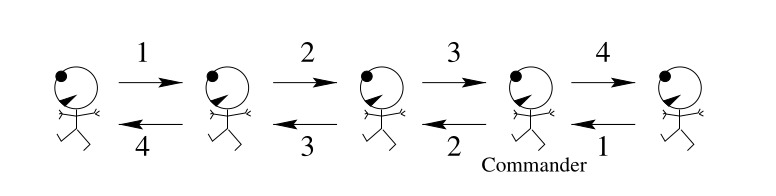
\includegraphics[width=\textwidth]{LinearTroop.png}
    \end{center}
    \caption{A line of soldiers counting themselves using
      message-passing rule-set A. The commander can add ``3'' from the
      soldier in front, ``1'' from the soldier behind, and ``1'' for
      himself, and deduce that there are 5 soldiers in total.}
  \end{figure}
\end{frame}


\begin{frame}{Message-passing rule-set A (parallel pseudo-code).}
  \begin{enumerate}
  \item If you are the front soldier in the line, say the number \textbf{one} to the
    soldier behind you.
  \item If you are the rearmost soldier in the line, say the number \textbf{one} to
    the soldier in front of you.
  \item If a soldier ahead of or behind you says a number to you, add one
    to it, and say the new number to the soldier on the other side.
  \end{enumerate}
\end{frame}

\begin{frame}[allowframebreaks]{Implementation}
  \begin{small}
    \lstinputlisting{MATLAB/soldiers.m}
  \end{small}
\end{frame}

\subsection{Tree graph topology}

\begin{frame}{General topology of the troop}
  \begin{figure}[H]
    \begin{figure}
      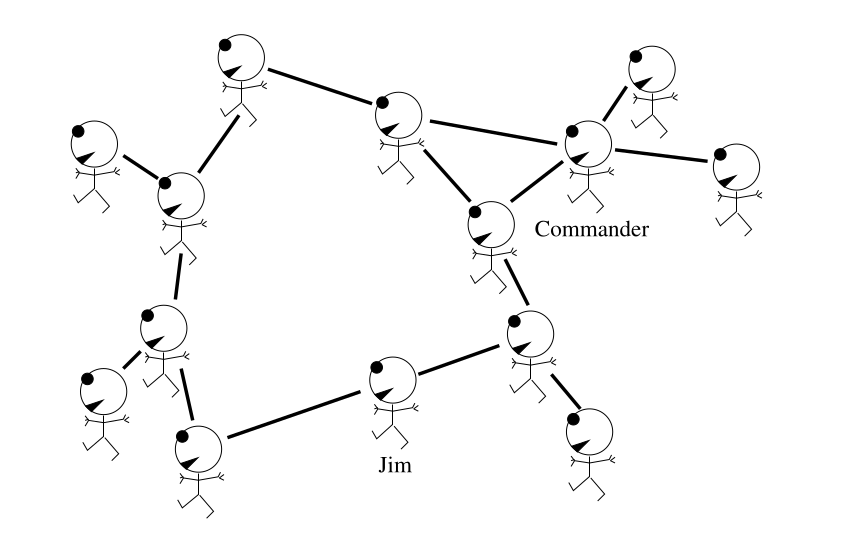
\includegraphics[width=\textwidth]{SwarmOfGuerillas.png}
    \end{figure}
    \caption{A swarm of guerillas.}
  \end{figure}
\end{frame}

\begin{frame}[allowframebreaks]{Arranging workers/labs into a graph}
  \begin{small}
    \lstinputlisting{MATLAB/buildTroop.m}
  \end{small}
\end{frame}  

\begin{frame}{A tree topology of the troop}
  \begin{figure}
    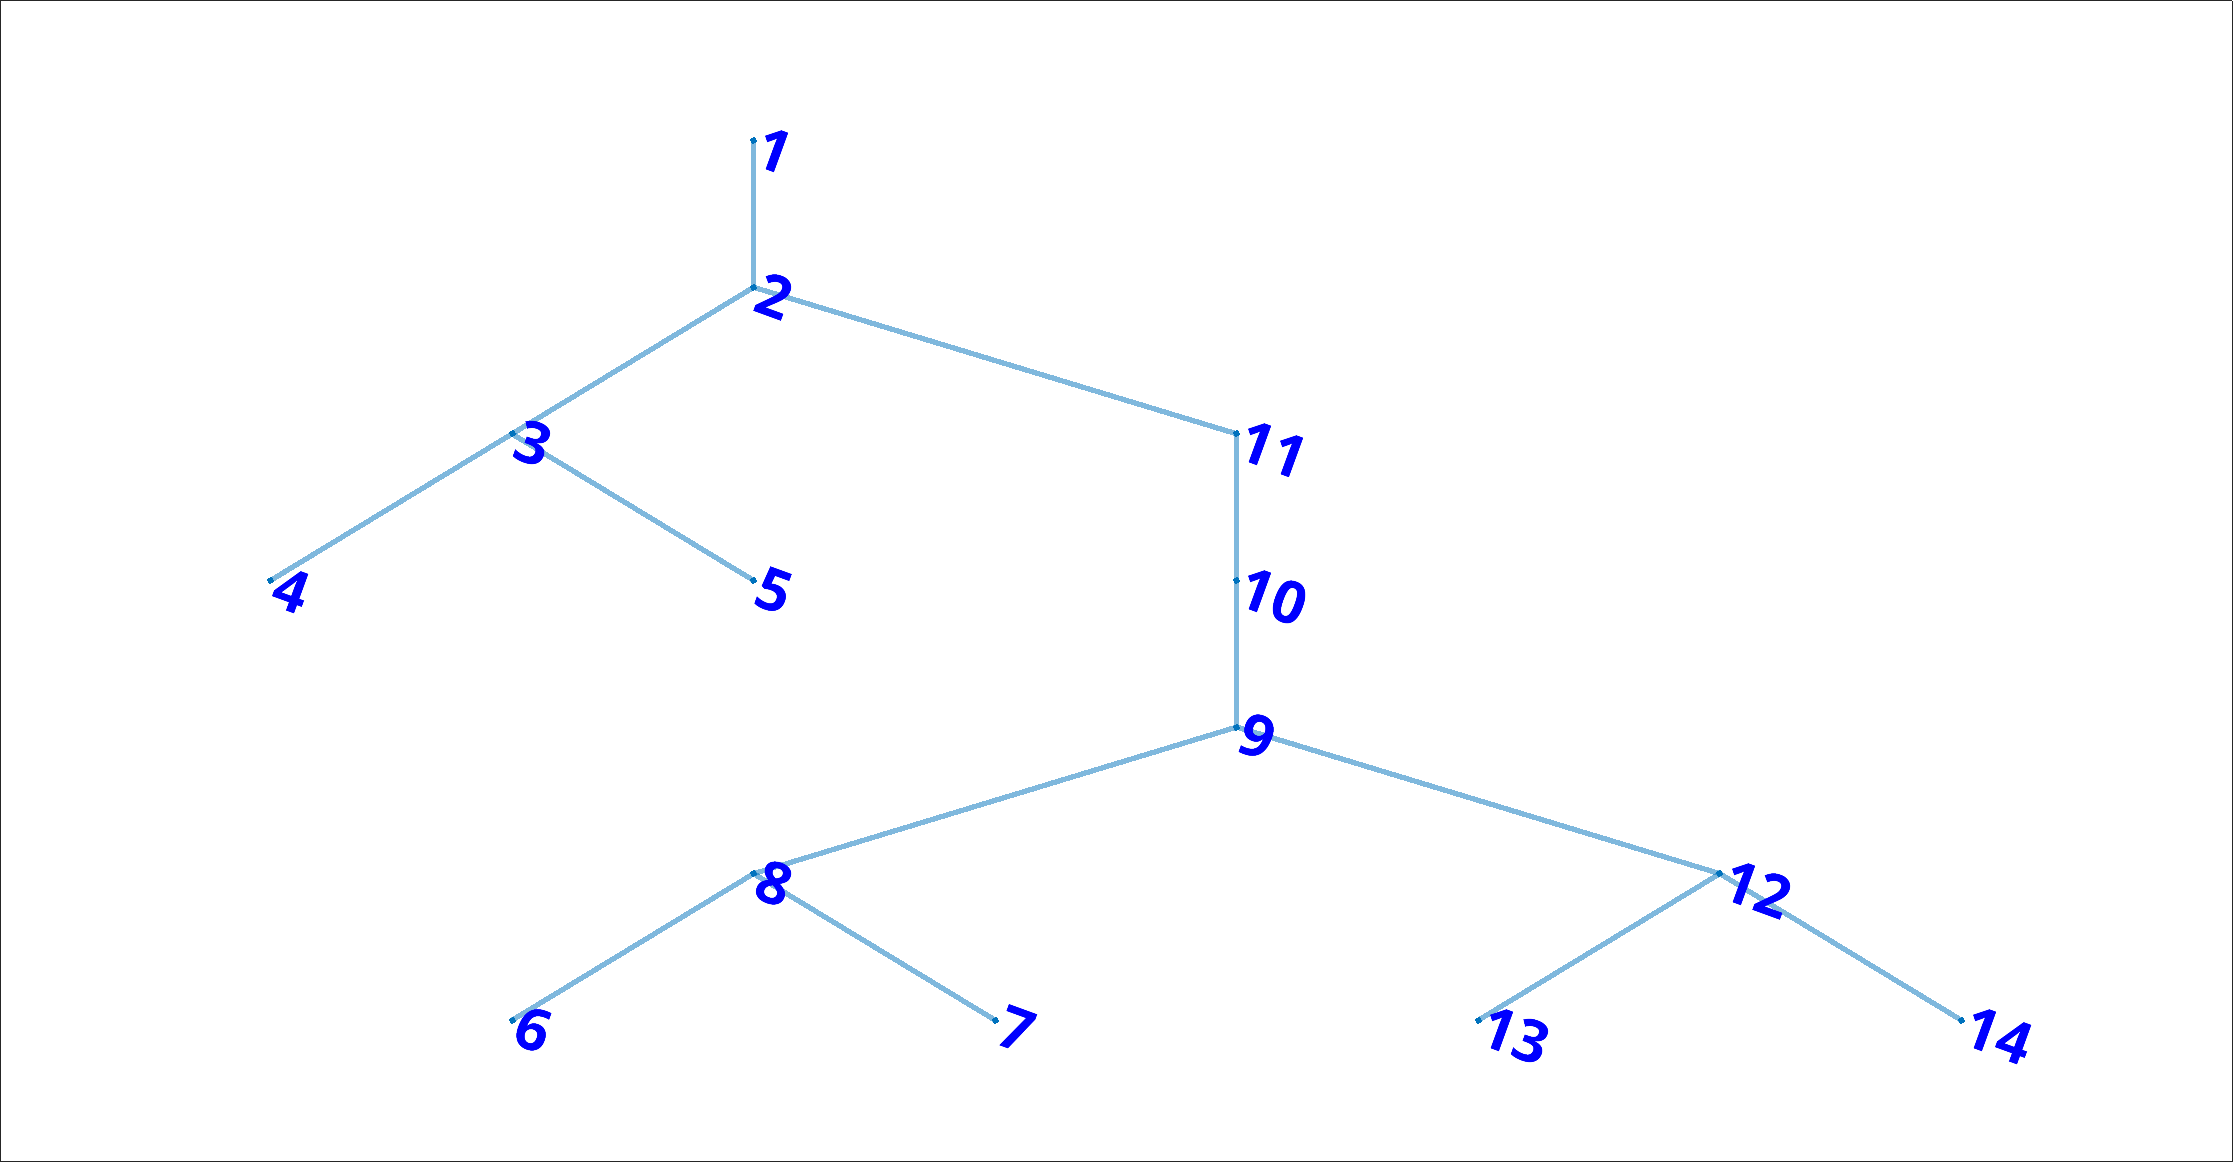
\includegraphics[width=\textwidth]{TroopTopology.png}
  \end{figure}
\end{frame}

\begin{frame}[allowframebreaks]{Message-passing rule-set B.}
  \begin{algorithmic}[1]
    \Procedure{MessagePassing}{$Graph$}
      \State $N \gets \text{the count your neighbours in $Graph$}$
      \State $m\gets 0$ \Comment{count of messages received from  neighbours}
      \For{$j$ from $1$ to $N$} 
        \State $v_j\gets -1$ \Comment{initial value of message is invalid}
      \EndFor
      \State $V\gets 0$ \Comment{running total of messages you have received}
      \If{$m == N - 1$}
        \State Find neighbor $j$ such that $v_j==-1$
        \Comment{the only one who has not sent you a message} 
        \State Tell them the number $V + 1$
      \EndIf
      \newpage
      \If{$V==N$}
        \State the number $V + 1$ is the required total.
        \For{ each neighbour $n$}
          \State say to neighbour $n$ the number $V + 1 - v_n$
        \EndFor
      \EndIf
    \EndProcedure
  \end{algorithmic}
\end{frame}

\subsection{Implementation}

\begin{frame}[allowframebreaks]{Implementation}
  \begin{small}
    \lstinputlisting{MATLAB/soldiers2.m}
  \end{small}
\end{frame}

\begin{frame}[allowframebreaks]{A modified implementation}
  \begin{small}
    \lstinputlisting{MATLAB/soldiers3.m}
  \end{small}
\end{frame}

\begin{frame}[allowframebreaks]{Sample output}
  \begin{tiny}
    \VerbatimInput{outputs/soldiers3_output.txt}
  \end{tiny}
\end{frame}

\section{Wrapping up}

\begin{frame}{What has been left out?}
  \begin{itemize}
  \item \emph{OpenMP} (e.g., GOMP=GNU OpenMP); a high
    level interface to threads (SPMD) and
    vectorization (SIMD); realized as C/Fortran compiler
    \emph{pragmas} (annotations)
  \item \emph{POSIX threads} (``pthreads''); a C library available on most OS
    which allows direct access to multi-threading and
    thread synchronization
  \item Extensive \emph{C++ language} constructs supporting parallelism
  \item \emph{Building hardware}; hardware is inherently parallel;
    the most straightforward hardware to build is FPGA (Field-Programmable Gate Arrays);
    programming languages \emph{Verilog} and \emph{VHDL}
  \item University of Arizona \emph{HPC facilities}
  \end{itemize}
\end{frame}


\end{document}
